\let\lesson\undefined
\newcommand{\lesson}{\phantomlesson{Ôn tập chương I}}
\chapter[Ôn tập chương I]{Ôn tập chương I}


\hdc{
	\section{}
	Mỗi câu trả lời đúng thí sinh được \textbf{0,25 điểm}.
	\begin{center}
		\begin{tabular}{|C{2.5cm}|C{4.0cm}|C{2.5cm}|C{4.0cm}|}
			\hline
			\thead{Câu} & \thead{Đáp án} & \thead{Câu} & \thead{Đáp án}\\
			\hline
			1 & C &  10 & A \\ 
			\hline
			2 & B &  11 & A \\ 
			\hline
			3 & A &  12 & A \\ 
			\hline
			4 & B &  13 & D \\ 
			\hline
			5 & A &  14 & B \\ 
			\hline
			6 & B &  15 & D \\ 
			\hline
			7 & C &  16 & B \\ 
			\hline
			8 & D &  17 & C \\ 
			\hline
			9 & A &  18 & C \\ 
			\hline
		\end{tabular}
	\end{center}
	\section{}
	Điểm tối đa của 01 câu hỏi là \textbf{1 điểm}.
	\begin{itemize}
		\item Thí sinh lựa chọn chính xác 01 ý trong 1 câu hỏi được \textbf{0,1} điểm.
		\item Thí sinh lựa chọn chính xác 02 ý trong 1 câu hỏi được \textbf{0,25} điểm.
		\item Thí sinh lựa chọn chính xác 03 ý trong 1 câu hỏi được \textbf{0,50} điểm.
		\item Thí sinh lựa chọn chính xác cả 04 ý trong 1 câu hỏi được \textbf{1} điểm.
	\end{itemize}
	\begin{center}
		\begin{tabular}{|C{1.0cm}|C{2.0cm}|C{3.0cm}|C{1.0cm}|C{2.0cm}|C{3.0cm}|}
			\hline
			\thead{Câu} & \thead{Lệnh hỏi} &\thead{Đáp án\\ (Đ/S)} &\thead{Câu} & \thead{Lệnh hỏi} &\thead{Đáp án\\ (Đ/S)}\\
			\hline
			\multirow{4}{*}{\textbf{1}}& a) & S & \multirow{4}{*}{\textbf{3}} & a) & Đ \\
			\cline{2-3}\cline{5-6}
			& b) & Đ &                             & b) & Đ \\
			\cline{2-3}\cline{5-6}
			& c) & S &                             & c) & S \\
			\cline{2-3}\cline{5-6}
			& d) & Đ &                             & d) & Đ \\
			\hline
			\multirow{4}{*}{\textbf{2}}& a) & Đ & \multirow{4}{*}{\textbf{4}} & a) & S \\
			\cline{2-3}\cline{5-6}
			& b) & Đ &                             & b) & Đ \\
			\cline{2-3}\cline{5-6}
			& c) & S &                             & c) & Đ \\
			\cline{2-3}\cline{5-6}
			& d) & S &                             & d) & S \\
			\hline		                           		                       
		\end{tabular}
	\end{center}
	\section{}
	Mỗi câu trả lời đúng thí sinh được \textbf{0,25 điểm}.
	\begin{center}
		\begin{tabular}{|C{2.5cm}|C{4.0cm}|C{2.5cm}|C{4.0cm}|}
			\hline
			\thead{Câu} & \thead{Đáp án} & \thead{Câu} & \thead{Đáp án}\\
			\hline
			1 & 8,3 &  4 & 25926 \\ 
			\hline
			2 & 5,43 &  5 & 0,96 \\ 
			\hline
			3 & 7 &  6 & 48,56\\ 
			\hline
		\end{tabular}
	\end{center}
	\newpage
}
\setcounter{section}{0}
\section{Câu trắc nghiệm nhiều phương án lựa chọn.}
\textit{Thí sinh trả lời từ câu 1 đến câu 18. Mỗi câu hỏi thí sinh chọn một phương án.}
\begin{enumerate}[label=\bfseries Câu \arabic*:, leftmargin=1.7cm]
	\item Quy ước dấu nào sau đây phù hợp với định luật I của nhiệt động lực học?
	\begin{mcq}
		\item Vật nhận công $A<0$; vật nhận nhiệt $Q<0$.
		\item Vật thực hiện công $A>0$; vật truyền nhiệt lượng $Q<0$.
		\item Vật nhận công $A>0$; vật nhận nhiệt lượng $Q>0$.
		\item Vật thực hiện công $A>0$; vật truyền nhiệt lượng $Q>0$.
	\end{mcq}
\hideall{
\textbf{Đáp án C.}
}

\item Ở nhiệt độ phòng, chất nào sau đây không tồn tại ở thể lỏng?
\begin{mcq}(4)
	\item Rượu.
	\item Nhôm.
	\item Thuỷ ngân.
	\item Nước.
\end{mcq}
\hideall{
\textbf{Đáp án B.}
}

\item Vật nào sau đây \textbf{không} có cấu trúc tinh thể?
\begin{mcq}(2)
	\item Chiếc cốc thuỷ tinh.
	\item Hạt muối ăn.
	\item Viên kim cương.
	\item Miếng thạch anh.
\end{mcq}
\hideall{
\textbf{Đáp án A.}
}

\item Điều nào sau đây là \textbf{sai} khi nói về sự đông đặc?
\begin{mcq}
	\item Sự đông đặc là quá trình chuyển từ thể lỏng sang thể rắn.
	\item Với một chất rắn, nhiệt độ đông đặc luôn nhỏ hơn nhiệt độ nóng chảy.
	\item Trong suốt quá trình đông đặc, nhiệt độ của vật không thay đổi.
	\item Nhiệt độ đông đặc của các chất thay đổi theo áp suất bên ngoài.
\end{mcq}
\hideall{
\textbf{Đáp án B.}
}

\item Biểu thức nào sau đây là biểu thức chuyển đổi đúng đơn vị nhiệt độ từ $\si{\celsius}$ sang thang $\si{\kelvin}$?
\begin{mcq}(2)
	\item $\xsi{T}{\left(\si{\kelvin}\right)}=\xsi{t}{\left(\si{\celsius}\right)}+273$.
	\item $\xsi{T}{\left(\si{\kelvin}\right)}=\xsi{t}{\left(\si{\celsius}\right)}-273$.
	\item $\xsi{T}{\left(\si{\kelvin}\right)}=\dfrac{9}{5}\xsi{t}{\left(\si{\celsius}\right)}+273$.
	\item $\xsi{T}{\left(\si{\kelvin}\right)}=\dfrac{9}{5}\xsi{t}{\left(\si{\celsius}\right)}-273$.
\end{mcq}
\hideall{
\textbf{Đáp án A.}
}

\item Trong thang nhiệt độ Celsius, nhiệt độ không tuyệt đối là
\begin{mcq}(4)
	\item $\SI{100}{\celsius}$.
	\item $\SI{-273}{\celsius}$.
	\item $\SI{0}{\celsius}$.
	\item $\SI{-32}{\celsius}$.
\end{mcq}
\hideall{
\textbf{Đáp án B.}
}

\item Đơn vị nhiệt nóng chảy riêng của vật rắn là
\begin{mcq}(4)
	\item $\si{\joule}$.
	\item $\si{\joule/\kelvin}$.
	\item $\si{\joule/\kilogram}$.
	\item $\si{\joule/\left(\kilogram\cdot\kelvin\right)}$.
\end{mcq}
\hideall{
\textbf{Đáp án C.}
}

\item Kết luận nào sau đây \textbf{không đúng} với thang nhiệt độ Celsius?
\begin{mcq}
	\item Đơn vị đo nhiệt độ là $\si{\celsius}$.
	\item Chọn mốc nhiệt độ nước đá đang tan ở áp suất $\SI{1}{atm}$ là $\SI{0}{\celsius}$.
	\item Chọn mốc nhiệt độ nước sôi ở áp suất $\SI{1}{atm}$ là $\SI{100}{\celsius}$.
	\item $\SI{1}{\celsius}$ tương ứng với $\SI{273}{\kelvin}$.
\end{mcq}
\hideall{
\textbf{Đáp án D.}
}

\item Nhiệt hoá hơi riêng của nước là $\SI{2.3E6}{\joule/\kilogram}$. Phát biểu nào dưới đây là \textbf{đúng}?
\begin{mcq}
	\item Mỗi kilogram nước cần thu một lượng nhiệt $\SI{2.3E6}{\joule}$ để bay hơi hoàn toàn ở nhiệt độ sôi và áp suất chuẩn.
	\item Mỗi kilogram nước cần thu một lượng nhiệt $\SI{2.3E6}{\joule}$ để bay hơi hoàn toàn.
	\item Mỗi kilogram nước cần toả ra một lượng nhiệt $\SI{2.3E6}{\joule}$ để bay hơi hoàn toàn ở nhiệt độ sôi.
	\item Một lượng nước bất kì cần thu một lượng nhiệt là $\SI{2.3E6}{\joule}$ để bay hơi hoàn toàn.
\end{mcq}
\hideall{
\textbf{Đáp án A.}
}

\item Hãy tìm ý \textbf{không đúng} với mô hình động học phân tử.
\begin{mcq}
	\item Tốc độ chuyển động của các phân tử cấu tạo nên vật càng lớn thì thể tích của vật càng lớn.
	\item Các chất được cấu tạo từ các hạt riêng biệt gọi là phân tử.
	\item Các phân tử chuyển động không ngừng.
	\item Giữa các phân tử có lực tương tác gọi là lực liên kết phân tử.
\end{mcq}
\hideall{
\textbf{Đáp án A.}
}

\item Điểm đóng băng và điểm sôi của nước theo thang nhiệt độ Kelvin là
\begin{mcq}(2)
	\item $\SI{273}{\kelvin}$ và $\SI{373}{\kelvin}$.
	\item $\SI{0}{\kelvin}$ và $\SI{100}{\kelvin}$.
	\item $\SI{73}{\kelvin}$ và $\SI{37}{\kelvin}$.
	\item $\SI{32}{\kelvin}$ và $\SI{212}{\kelvin}$.
\end{mcq}
\hideall{
\textbf{Đáp án A.}
}

\item Người ta cung cấp cho khí trong một cylanh nằm ngang nhiệt lượng $\SI{2}{\joule}$. Đồng thời nén piston một đoạn $\SI{5}{\centi\meter}$ với một lực có độ lớn là $\SI{20}{\newton}$. Độ biến thiên nội năng của khí là
\begin{mcq}(4)
	\item $\SI{3}{\joule}$.
	\item $\SI{1}{\joule}$.
	\item $\SI{-1}{\joule}$.
	\item $\SI{-3}{\joule}$.
\end{mcq}
\hideall{
\textbf{Đáp án A.}\\
$$\Delta U=Q+A=Q+F\cdot s=\SI{3}{\joule}.$$
}

\item Nhiệt lượng cần cung cấp cho $\SI{0.5}{\kilogram}$ nước ở $\SI{0}{\celsius}$ đến khi nó sôi là bao nhiêu? Biết nhiệt dung riêng của nước là $\SI{4180}{\joule/\left(\kilogram\cdot\kelvin\right)}$.
\begin{mcq}(4)
	\item $\SI{5E5}{\joule}$.
	\item $\SI{3E5}{\joule}$.
	\item $\SI{4.18E5}{\joule}$.
	\item $\SI{2.09E5}{\joule}$.
\end{mcq}
\hideall{
\textbf{Đáp án D.}\\
$$Q=mc\Delta t=\SI{2.09E5}{\joule}.$$
}

\item Biết nhiệt dung riêng của nước là $\SI{4200}{\joule/\left(\kilogram\cdot\kelvin\right)}$, nhiệt nóng chảy riêng của nước đá là $\SI{3.4E5}{\joule/\kilogram}$. Nhiệt lượng cần cung cấp cho $\SI{2}{\kilogram}$ nước đá ở nhiệt độ $\SI{0}{\celsius}$ là bao nhiêu để tăng nhiệt độ lên $\SI{60}{\celsius}$ là
\begin{mcq}(4)
	\item $\SI{0.72E6}{\joule}$.
	\item $\SI{1.184E6}{\joule}$.
	\item $\SI{2.254E6}{\joule}$.
	\item $\SI{1.548E6}{\joule}$.
\end{mcq}
\hideall{
\textbf{Đáp án B.}\\
Nhiệt lượng cần cung cấp cho $\SI{2}{\kilogram}$ nước đá ở nhiệt độ $\SI{0}{\celsius}$ là bao nhiêu để chuyển lên nhiệt độ $\SI{60}{\celsius}$ là
$$Q=m\lambda+mc\Delta t=\SI{1.184E6}{\joule}.$$
}

\item Một lượng nước và một lượng rượu có thể tích bằng nhau, được cung cấp các nhiệt lượng tương ứng là $Q_1$ và $Q_2$. Biết khối lượng riêng của nước là $\SI{1000}{\kilogram/\meter^3}$ và của rượt là $\SI{800}{\kilogram/\meter^3}$, nhiệt dung riêng của nước và rượu lần lượt là $\SI{4200}{\joule/\left(\kilogram\cdot\kelvin\right)}$ và $\SI{2500}{\joule/\left(\kilogram\cdot\kelvin\right)}$. Để độ tăng nhiệt độ của nước và rượu bằng nhau thì
\begin{mcq}(4)
	\item $Q_1=Q_2$.
	\item $Q_1=1,68Q_2$.
	\item $Q_1=1,25Q_2$.
	\item $Q_1=2,10Q_2$.
\end{mcq}
\hideall{
\textbf{Đáp án D.}\\
$$\dfrac{Q_1}{Q_2}=\dfrac{m_1c_1}{m_2c_2}=\dfrac{\rho_1c_1}{\rho_2c_2}=2,1.$$
}

\item Một ấm đun nước bằng nhôm có khối lượng $\SI{400}{\gram}$, chứa 3 lít nước được đun trên bếp. Khi nhận nhiệt lượng $\SI{740}{\kilo\joule}$ thì ấm đạt đến nhiệt độ $\SI{80}{\celsius}$. Biết nhiệt dung riêng của nhôm là $\SI{880}{\joule/\left(\kilogram\cdot\kelvin\right)}$, nhiệt dung riêng của nước là $\SI{4190}{\joule/\left(\kilogram\cdot\kelvin\right)}$. Coi nhiệt lượng mà ấm toả ra bên ngoài là không đáng kể. Nhiệt độ ban đầu của ấm và nước là
\begin{mcq}(4)
	\item $\SI{45.2}{\celsius}$.
	\item $\SI{22.7}{\celsius}$.
	\item $\SI{37.2}{\celsius}$.
	\item $\SI{16.7}{\celsius}$.
\end{mcq}
\hideall{
\textbf{Đáp án B.}\\
$$\Delta t=\dfrac{Q}{m_1c_1+m_2c_2}=\SI{57.27}{\celsius}\Rightarrow t_0=\SI{22.7}{\celsius}.$$
}

\item Người ta thực hiện công $\SI{100}{\joule}$ để nén khí trong một cylanh. Biết khí truyền ra môi trường xung quanh nhiệt lượng $\SI{30}{\joule}$ thì độ biến thiên nội năng của khí là
\begin{mcq}(4)
	\item $\SI{30}{\joule}$.
	\item $\SI{130}{\joule}$.
	\item $\SI{70}{\joule}$.
	\item $\SI{100}{\joule}$.
\end{mcq}
\hideall{
\textbf{Đáp án C.}\\
Độ biến thiên nội năng của khí:
$$\Delta U=A+Q=\SI{100}{\joule}-\SI{30}{\joule}=\SI{70}{\joule}.$$
}

\item Một lượng khí khi bị nung nóng đã tăng thể tích thêm $\SI{0.02}{\meter^3}$ và nội năng biến thiên $\SI{1280}{\joule}$. Biết trong quá trình thay đổi thể tích thì áp suất khí luôn bằng $\SI{2E5}{\pascal}$. Nhiệt lượng đã truyền cho khí là
\begin{mcq}(4)
	\item $\SI{2720}{\joule}$.
	\item $\SI{1280}{\joule}$.
	\item $\SI{5280}{\joule}$.
	\item $\SI{4000}{\joule}$.
\end{mcq}
\hideall{\textbf{Đáp án C.}\\
Công khối khí thực hiện trong quá trình dãn nở:
$$A'=F\cdot \Delta x=pS\Delta x=p\Delta V=\SI{4000}{\joule}.$$
Nhiệt lượng mà khí đã nhận:
$$Q=\Delta U-A=\Delta U+A'=\SI{5280}{\joule}.$$
}
\end{enumerate}
\section{Câu trắc nghiệm đúng/sai.} 
\textit{Thí sinh trả lời từ câu 1 đến câu 4. Trong mỗi ý \textbf{a)}, \textbf{b)}, \textbf{c)}, \textbf{d)} ở mỗi câu, thí sinh chọn đúng hoặc sai.}
\begin{enumerate}[label=\bfseries Câu \arabic*:, leftmargin=1.7cm]

	\item Nhận định về các phát biểu sau khi nói về đặc điểm của các chất rắn, lỏng, khí.
	\begin{enumerate}[label=\alph*)]
		\item Các phân tử ở thể lỏng có khoảng cách giữa các phân tử nhỏ hơn khi ở thể rắn.
		\item Các phân tử trong thể khí tự do di chuyển và không bị ràng buộc bởi lực tương tác giữa chúng.
		\item Vật ở thể lỏng không có thể tích riêng, nhưng có hình dạng riêng.
		\item Vật ở thể rắn có thể tích và hình dạng riêng, rất khó nén.
	\end{enumerate}
	\hideall{
		\begin{enumerate}
			\item Sai. Các phân tử thể lỏng có khoảng cách giữa các phân tử lớn hơn khi ở thể rắn.
			\item Sai. Có lực tương tác phân tử nhưng rất yếu.
			\item Sai. Vật ở thể lỏng có thể tích riêng, nhưng không có hình dạng riêng.
			\item Đúng.
		\end{enumerate}
	}

\item Nhận định các phát biểu sau về nội năng của một hệ.
\begin{enumerate}[label=\alph*)]
	\item Nội năng của một vật phụ thuộc vào nhiệt độ và thể tích của vật.
	\item Nội năng của một vật thay đổi trong quá trình truyền nhiệt và trong quá trình thực hiện công.
	\item Nội năng của vật A lớn hơn nội năng của vật B thì nhiệt độ của vật A lớn hơn nhiệt độ của vật B.
	\item Nội năng có thể chuyển hoá hoàn toàn thành cơ năng.
\end{enumerate}
\hideall{
\begin{enumerate}[label=\alph*)]
	\item Đúng.
	\item Đúng.
	\item Sai. Nội năng của hệ không chỉ phụ thuộc vào nhiệt độ của hệ mà còn phụ thuộc vào thể tích của hệ.
	\item Sai. Nội năng của hệ không thể chuyển hoá hoàn toàn thành cơ năng.
\end{enumerate}
}


\item Một động cơ nhiệt lý tưởng hoạt động giữa hai nguồn nhiệt $\SI{100}{\celsius}$ và $\SI{24.5}{\celsius}$ thì thực hiện công $\SI{2}{\kilo\joule}$.
\begin{enumerate}[label=\alph*)]
	\item Hiệu suất của động cơ là $\SI{0.2}{}$.
	\item Nhiệt lượng động cơ nhận từ nguồn nóng là $\SI{0.1}{\kilo\joule}$.
\item Nhiệt lượng động cơ cung cấp cho nguồn lạnh là $\SI{1.9}{\kilo\joule}$.
	\item Để động cơ đạt hiệu suất $\SI{30}{\percent}$ thì phải tăng nhiệt độ nguồn nóng lên $\SI{152}{\celsius}$.
\end{enumerate}
\hideall{\begin{enumerate}[label=\alph*)]
		\item Đúng.
		\item Đúng.
		\item Sai. Nhiệt lượng động cơ cung cấp cho nguồn lạnh là $\SI{7.88}{\kilo\joule}$.
		\item Đúng. 
	\end{enumerate}
}
	
	
	\item Dùng bếp điện để đun một ấm nhôm khối lượng $\SI{600}{\gram}$ đựng $\SI{1.5}{\text{lít}}$ nước ở nhiệt độ $\SI{20}{\celsius}$. Sau $\SI{35}{\minute}$ đã có $\SI{20}{\percent}$ lượng nước trong ấm hoá hơi ở nhiệt độ sôi $\SI{100}{\celsius}$. Biết có $\SI{60}{\percent}$ nhiệt lượng mà bếp toả ra được dùng vào việc đun ấm nước. Cho nhiệt dung riêng của nhôm là $\SI{880}{\joule/\left(\kilogram\cdot\kelvin\right)}$, của nước là $\SI{4200}{\joule/\left(\kilogram\cdot\kelvin\right)}$, nhiệt hoá hơi riêng của nước ở nhiệt độ sôi $\SI{100}{\celsius}$ là $\SI{2.26E6}{\joule/\kilogram}$ và khối lượng riêng của nước là $\SI{1}{\kilogram/\text{lít}}$.
	\begin{enumerate}[label=\alph*)]
		\item Nhiệt lượng cần thiết để đun ấm nước từ $\SI{20}{\celsius}$ đến $\SI{100}{\celsius}$ là $\SI{504000}{\joule}$.
		\item Khối lượng nước đã hoá hơi là $\SI{0.03}{\kilogram}$.
		\item Nhiệt lượng mà bếp điện cung cấp để đun nước đến khi sôi là $\SI{910.4}{\kilo\joule}$.
		\item Nhiệt lượng trung bình mà bếp điện cung cấp cho ấm nước trong mỗi giây là $\SI{582.97}{\joule}$.
	\end{enumerate}
\hideall{
\begin{enumerate}[label=\alph*)]
	\item Sai. Nhiệt lượng cần thiết để đun sôi ấm nước là $\SI{546240}{\joule}$.
	\item Đúng.
	\item Đúng.
	\item Sai. Nhiệt lượng trung bình mà bếp điện cung cấp cho ấm nước trong mỗi giây là $\SI{971.6}{\joule}$.
\end{enumerate}
}
\end{enumerate}
\section{Câu trắc nghiệm trả lời ngắn.} \textit{Thí sinh trả lời từ câu 1 đến câu 6.}
\begin{enumerate}[label=\bfseries Câu \arabic*:, leftmargin=1.7cm]
	\item Giả sử rằng các tuabin ở nhà máy nhiệt điện đã được nâng cấp, dẫn đến sự cải thiện về hiệu suất $\SI{3.32}{\percent}$. Biết rằng trước khi nâng cấp thì hiệu suất của nhà máy điện là $\SI{36}{\percent}$, nhiệt lượng truyền vào động cơ trong một ngày vẫn không đổi và bằng $\SI{2.5E14}{\joule}$. Có thêm bao nhiêu lượng điện năng được sản xuất trong 1 ngày nhờ vào sự nâng cấp trên \textit{(tính theo đơn vị  $\SI{E12}{\joule}$)}?
	\hideall{
$$\Delta A=Q_1\Delta H=\left(\SI{2.5E14}{\joule}\right)\cdot\left(\SI{3.32}{\percent}\right)=\SI{8.3E12}{\joule}.$$
}
	
	\item Người ta thả một miếng đồng khối lượng $\SI{0.5}{\kilogram}$ vào $\SI{500}{\gram}$ nước. Miếng đồng nguội đi từ $\SI{80}{\celsius}$ xuống $\SI{20}{\celsius}$. Hỏi nước nóng lên thêm bao nhiêu $\si{\celsius}$ \textit{(làm tròn đến 2 số thập phân)}? Biết nhiệt dung riêng của đồng là $\SI{380}{\joule/\left(\kilogram\cdot\kelvin\right)}$, nhiệt dung riêng của nước là $\SI{4200}{\joule/\left(\kilogram\cdot\kelvin\right)}$.
	\hideall{
		$$\Delta t=\dfrac{m_\text{đ}c_\text{đ}\left(80-20\right)}{m_\text{n}c_\text{n}}\approx\SI{5.43}{\celsius}.$$
}

\item Một ấm điện có công suất $\SI{1000}{\watt}$. Tính thời gian cần thiết để đun sôi $\SI{0.5}{\text{lít}}$ nước có nhiệt độ ban đầu là $\SI{20}{\celsius}$ ở áp suất tiêu chuẩn theo đơn vị phút. Bỏ qua sự trao đổi nhiệt với vỏ ấm và môi trường. Cho hiệu suất ấm đun là $\SI{40}{\percent}$. Biết nhiệt dung riêng của nước là $\SI{4200}{\joule/\left(\kilogram\cdot\kelvin\right)}$ và khối lượng riêng của nước là $\SI{1}{\kilogram/\liter}$.
\hideall{
$$t=\dfrac{mc\Delta t}{H\calP}\approx\SI{7}{\minute}.$$
}

\item Tính nhiệt lượng cần cung cấp \textit{(theo đơn vị $\si{\kilo\joule})$} cho $\SI{10}{\kilogram}$ nước ở $\SI{30}{\celsius}$ chuyển thành hơi ở $\SI{100}{\celsius}$. Cho biết nhiệt dung riêng của nước $\SI{4180}{\joule/\left(\kilogram\cdot\kelvin\right)}$ và nhiệt hoá hơi riêng của nước là $\SI{2.3E6}{\joule/\kilogram}$.
\hideall{
$$Q=mc\Delta t+mL=\SI{25926}{\kilo\joule}.$$
}
\\
\begin{minipage}[l]{0.7\textwidth}
	\item 10 viên nước đá được dùng để làm lạnh cốc nước soda có khối lượng $\SI{0.25}{\kilogram}$, mỗi viên đá có khối lượng $\SI{6}{\gram}$. Ban đầu, nước soda trong cốc có nhiệt độ $\SI{20}{\celsius}$. Xác định nhiệt độ cốc nước khi đá tan hết theo đơn vị $\si{\celsius}$ và làm tròn đến 2 chữ số thập phân. Biết rằng nhiệt dung riêng của nước là $\SI{4186}{\joule/\left(\kilogram\cdot\kelvin\right)}$, nhiệt nóng chảy riêng của nước đá là $\SI{3.34E5}{\joule/\kilogram}$. Bỏ qua sự trao đổi nhiệt với cốc và môi trường bên ngoài.
\end{minipage}\hfill
\begin{minipage}[l]{0.3\textwidth}
\begin{center}
	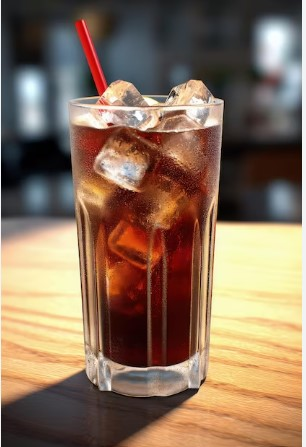
\includegraphics[width=0.3\linewidth]{../figs/VN12-Y24-PH-SYL-008-1}
\end{center}
\end{minipage}
\hideall{Khi có cân bằng nhiệt, tổng nhiệt lượng trao đổi trong hệ bằng 0:
	$$10m_\text{đ}\lambda+m_\text{n}c_\text{n}\left(t_\text{cb}-t_0\right)=0$$
$$\Rightarrow t_\text{cb}\approx\SI{0.69}{\celsius}.$$
}

\item Năm 1986, một tảng băng khổng lồ đã tách ra khỏi thềm băng Ross ở Nam Cực. Tảng băng có dạng gần như hình hộp chữ nhật với chiều dài $\SI{160}{\kilo\meter}$, chiều rộng $\SI{40}{\kilo\meter}$ và dày $\SI{250}{\meter}$. Khối lượng riêng của băng là $\SI{917}{\kilogram/\meter^3}$, nhiệt nóng chảy riêng của băng là $\SI{3.34E5}{\joule/\kilogram}$. Chỉ riêng ánh sáng Mặt Trời thì phải mất bao nhiêu năm để làm tan chảy được lớp băng dày như thế \textit{(làm tròn đến 2 chữ số thập phân)}. Cho rằng công suất toả nhiệt trung bình của Mặt Trời là $\SI{100}{\watt/\meter^2}$ và Mặt Trời chiếu sáng $\SI{12}{\hour}$ mỗi ngày.
\hideall{
	Nhiệt lượng cần cung cấp để làm tan khối băng:
	$$Q=\rho V\lambda=Sh\rho\lambda.$$
	Nhiệt lượng do Mặt Trời cung cấp:
	$$Q=\calP t$$
	Thời gian cần để băng tan:
	$$t=\dfrac{\rho h\lambda}{\calP}=\SI{212693}{\hour}.$$
	Mỗi ngày trung bình Mặt Trời chiếu sáng $\SI{12}{\hour}$ nên nếu chỉ riêng Mặt Trời chiếu sáng thì phải mất:
	$$\dfrac{t}{12\cdot 365}\approx\SI{48.56}{\text{năm}}.$$
}
\end{enumerate}
\begin{center}
	\textbf{--- HẾT ---}
\end{center}
